\documentclass[a4paper, oneside, openany, dvipsnames, table, 12pt]{article}
\usepackage[italian,british]{babel}
\usepackage{../../../Template/AFKstyleEng}
\usepackage{hyperref}
\usepackage{amsmath}
\usepackage{verbatim}
\newcommand{\Titolo}{Developer Manual}

\newcommand{\Gruppo}{TeamAFK}

\newcommand{\Redattori}{Simone Federico Bergamin \newline Olivier Utshudi}

\newcommand{\Verificatori}{}

\newcommand{\pathimg}{../Developer_manual/img/logoAFK.png}

\newcommand{\Approvatore}{}

\newcommand{\Distribuzione}{Prof. Vardanega Tullio \newline Prof. Cardin Riccardo \newline TeamAFK}

\newcommand{\Uso}{External}

\newcommand{\NomeProgetto}{Predire in Grafana}

\newcommand{\Mail}{gruppoafk15@gmail.com}

\newcommand{\Versionedoc}{1.0.0}

\newcommand{\DescrizioneDoc}{Developer manual made by \textit{TeamAFK} for the project \textit{Predire in Grafana}.}

\makeindex

\begin{document}
\frontispiece{}

%------------------ COLORI TABELLE 
\definecolor{pari}{RGB}{255, 207, 158} %{HTML}{E1F5FE} %azzurrino
\definecolor{dispari}{HTML}{FAFAFA} %bianco/grigetto 

%definizione colori per tabelle (tranne copertina)
\definecolor{redafk}{RGB}{255, 133, 51}
\definecolor{grey2}{RGB}{204, 204, 204}
\definecolor{greyRowafk}{RGB}{234, 234, 234}
\definecolor{lastrowcolor}{RGB}{176, 196, 222} %steel blue %{255,165,0} orange %{RGB}{255, 207, 158}
\rowcolors{2}{pari}{dispari}
\renewcommand{\arraystretch}{1.5}

%------------------

\newpage
\section*{Changelog}
\begin{longtable}{c c C{3.5cm} C{4cm} C{3cm}}
		\rowcolor{redafk}
\textcolor{white}{\textbf{Version}} & 
\textcolor{white}{\textbf{Date}} & 
\textcolor{white}{\textbf{Description}} & 
\textcolor{white}{\textbf{Name}} & 
\textcolor{white}{\textbf{Role}}\\
		\endfirsthead
		\rowcolor{redafk}
\textcolor{white}{\textbf{Version}} & 
\textcolor{white}{\textbf{Date}} & 
\textcolor{white}{\textbf{Description}} & 
\textcolor{white}{\textbf{Name}} & 
\textcolor{white}{\textbf{Role}}\\
		\endhead
		1.0.0 & 2020-06-10 & Document approved for RQ & Olivier Utshudi & \textit{Manager}\\
		0.7.0 & 2020-06-04 & Writed and checked section \S 7 - \S A & Davide Zilio \newline Fouad Farid & \textit{Programmer} \newline \textit{Verifier} \\
		0.6.0 & 2020-06-04 & Writed and checked section \S 6  & Simone Federio Bergamin \newline Fouad Farid & \textit{Programmer} \newline \textit{Verifier} \\
		0.4.0 & 2020-06-04 & Writed and checked section \S 5 & Olivier Utshudi \newline Simone Meneghin & \textit{Programmer} \newline \textit{Verifier} \\
		0.3.0 & 2020-06-04 & Writed and checked section \S 4 & Simone Federico Bergamin \newline Simone Meneghin & \textit{Programmer}\newline \textit{Verifier}\\
		0.2.0 & 2020-06-03 & Writed and checked sections \S 2- \S 3 & Olivier Utshudi \newline Simone Meneghin & \textit{Programmer}\newline \textit{Verifier}\\
		0.1.0 & 2020-06-03 & Writed and checked section \S 1 & Simone Federico Bergamin \newline Fouad Farid & \textit{Programmer}\newline \textit{Verifier}
	\end{longtable}

%Didascalia tabelle/immagini (prendono come riferimento la subsection)
\counterwithin{table}{subsection}
\counterwithin{figure}{subsection}
\newpage

%indice, indice figure e indice tabelle
\tableofcontents
\newpage
\listoffigures
\newpage
%\listoftables
\newpage

\section{Introduction}

\subsection{General description}
This document is “Predire in Grafana”’s user manual, a project developed by “Team AFK” for use on the Grafana\glo platform.

\subsection{Purpose of the document}
This document’s purpose is to demonstrate how to use Predire in Grafana’s two software components: the training tool and the prediction plug-in for Grafana itself.

\subsection{Predire in Grafana’s Purpose}
Predire in Grafana is a platform which allows users to train linear regression or support vector machine algorithms using machine learning\glo, and then use these algorithms to monitor and predict the behaviour of various systems of their choosing.
In more detail:	
Users can supply a CSV file to the training tool and receive a JSON file containing values which can then be used to set and calibrate SVM\glo or RL\glo algorithms by coupling the values contained in the JSON file with data streams coming from a database.

\subsection{Glossary}
At the end of the document an appendix is available where explanations for new or ambiguous terms can be found. These are marked with a subscript G.


\pagebreak
\section{System Requirements}
Here the requirements for use of the product are listed.

\subsection{Minimum Hardware Requirements}
Here the requirements for use of the product are listed.
\begin{itemize}
	\item 2GB of RAM;
	\item 5GB of space on a drive;
	\item Dual core processor.	
\end{itemize}

\subsection{Compatible Operating Systems}
The software was developed and tested on the following:
\begin{itemize}
	\item Windows 10;
	\item MacOS 10.15;
	\item Ubuntu 18, 20.
\end{itemize}

\subsection{Compatible Browsers}
Predire in Grafana can be accessed through the following browsers:
\begin{itemize}
	\item Google Chrome version 58 or newer;
	\item Mozilla Firefox version 54 or newer;
	\item Apple Safari version 10 or newer;
	\item Microsoft Edge version 14 or newer;
	\item Opera version 55 or newer.
\end{itemize}




\pagebreak
\section{The Training Tool}
Here the appropriate way of using the training tool is explained in detail.

\subsection{Access}
The tool is hosted by a web page and can thus be accessed via browser.

\subsection{Uploading a CSV File in the Tool}
The user will need to feed the tool a CSV file containing properly marked values for the algorithm the user has intention of training.

This can be done by selecting the "Selezionare il file" button, which will open a window from which the user will be able to select the CSV file he has intention of uploading.

\begin{figure}[H]
\centering
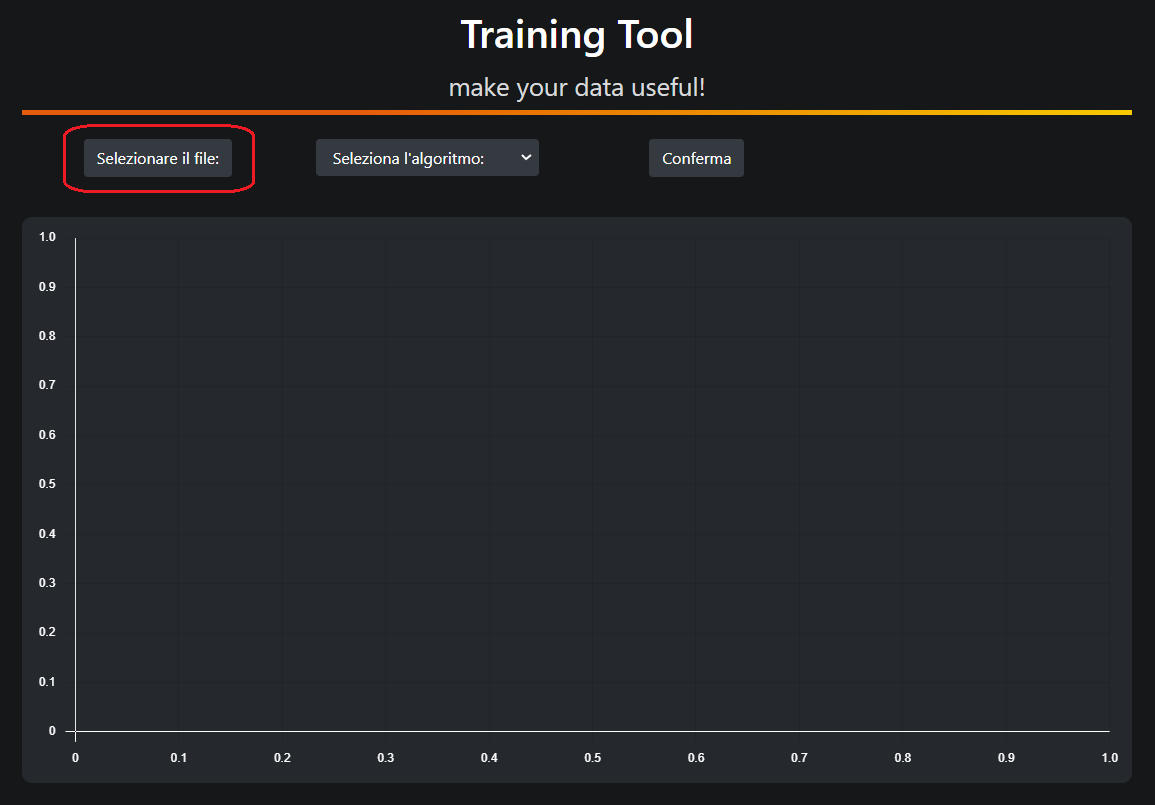
\includegraphics[scale=0.65]{img/tool/pointer_tool_1.png}
\caption{CSV-File selector}
\end{figure}
\newpage

\subsection{Selection of the Algorithm}
The user will then have to choose between training a support vector machine or a linear regression algorithm with the CSV file he has given to the tool.

To do this, the user can open a drop-down menu called "seleziona l'algoritmo" which displays the two algorithms that can be chosen, the preferred algorithm can at this point be selected.
\begin{figure}[H]
\centering
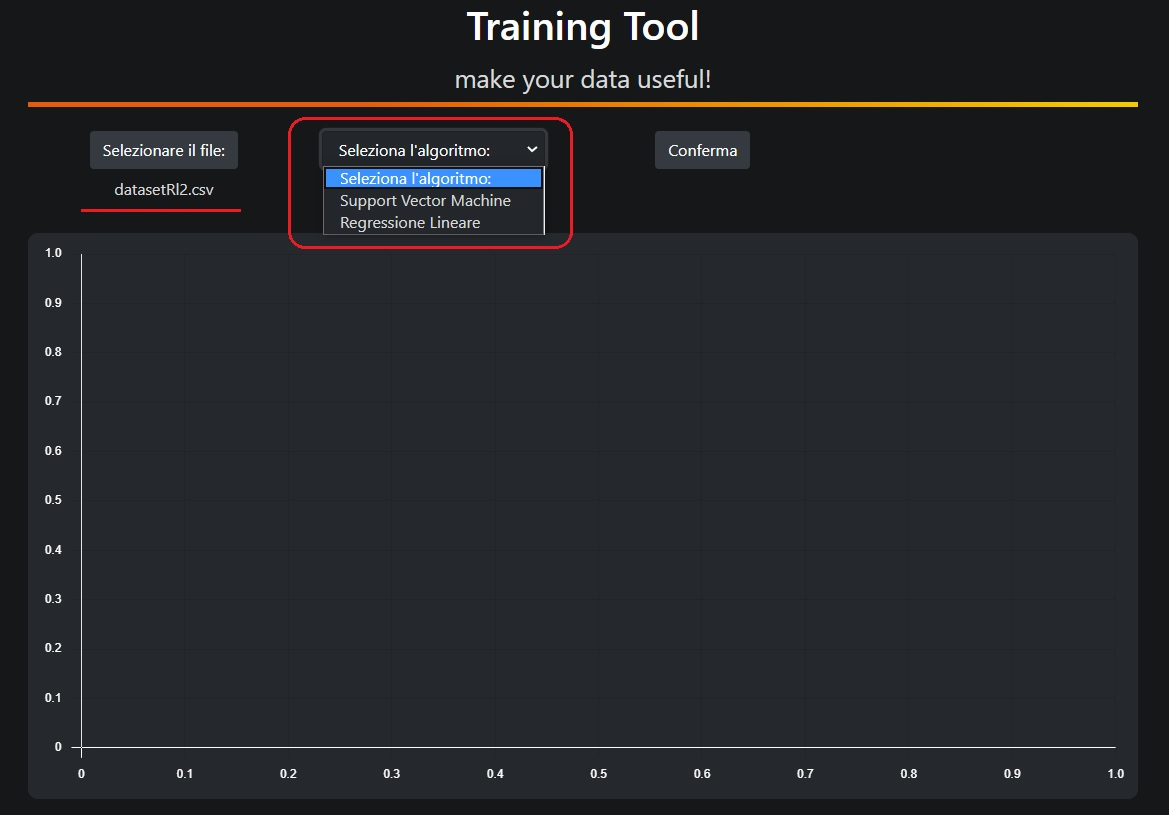
\includegraphics[scale=0.65]{img/tool/algo_selector.jpg}
\caption{Training algorithm selector}
\end{figure}
Should the user have uploaded training data incompatible with the selected algorithm, an error message will be displayed on selection of the "Conferma" button.\newline
\begin{figure}[H]
\centering

\includegraphics[scale=0.65]{img/tool/err_msg_algo.jpg}
\caption{Incompatible algorithm uploaded}
\end{figure}
\newpage
\subsection{Training Operation}
The tool will now be able to perform the training operation by simply  having the user select the “Conferma” button. The tool will now have produced a JSON file containing the values needed for use in the plug-in.
\begin{figure}[H]
\centering
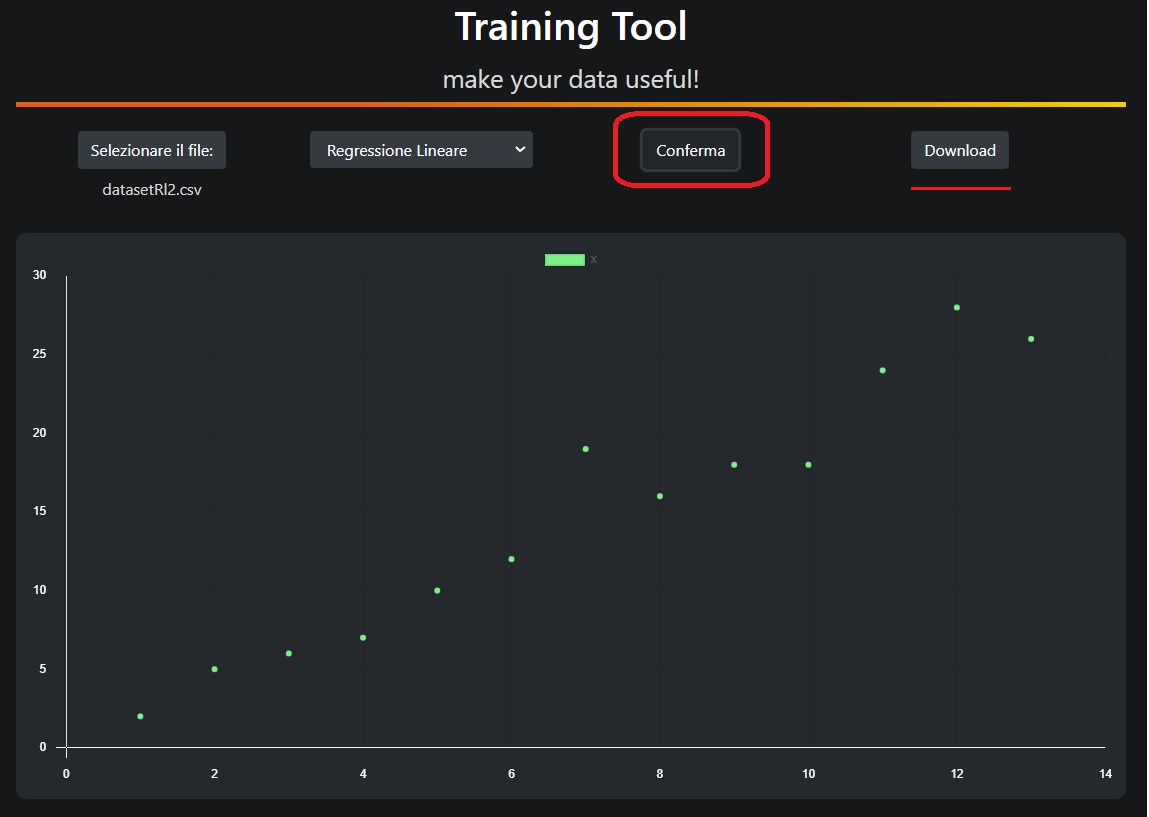
\includegraphics[scale=0.65]{img/tool/confirm.jpg}
\caption{Training operation with graphic point}
\end{figure}

A message will be displayed on selection of the "Conferma " button if the training operation is successfully completed
\newline
\begin{figure}[H]
\centering
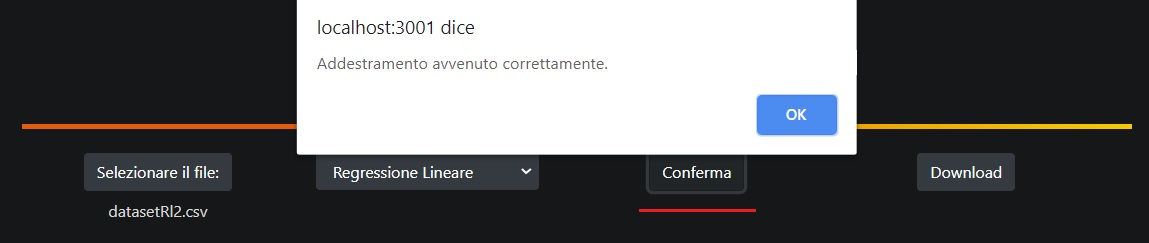
\includegraphics[scale=0.65]{img/tool/ok_msg.jpg}
\caption{Training operation is successfully completed}
\end{figure}  

\subsection{Obtaining the JSON File}
The user can now select the “download” button, which will only appear once the training operation has ended succesfully, and receive the JSON file.
\begin{figure}[H]
\centering
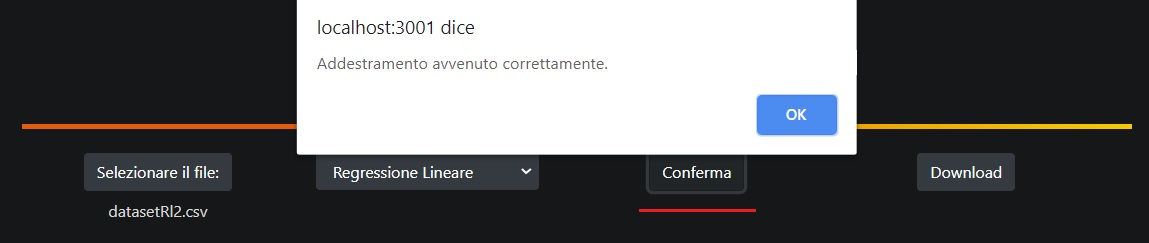
\includegraphics[scale=0.65]{img/tool/ok_msg.jpg}
\caption{The "Download" button is then clickable}
\end{figure} 

\pagebreak
\section{The plug-in}
Here a step by step explanation will guide the user through the proper usage of the preditcion plug-in.

\subsection{Loading the plug-in}
\begin{enumerate}
	\item The user will have to select the plus icon from the sidebar, from which a drop-down menu containing four options will appear; from this menu the “dashboard” option has to be selected;


\begin{figure}[H]
\centering
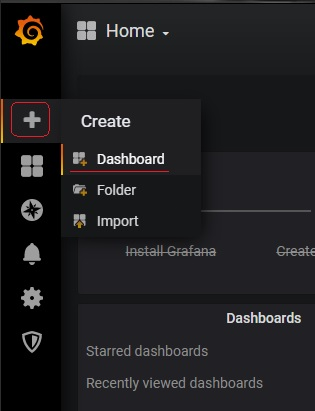
\includegraphics[scale=0.90]{img/plug-in/plus_dash.jpg}
\caption{Training operation with graphic point}
\end{figure}


	\item The user will now have to select the “Chose Visualization” button;


\begin{figure}[H]
\centering
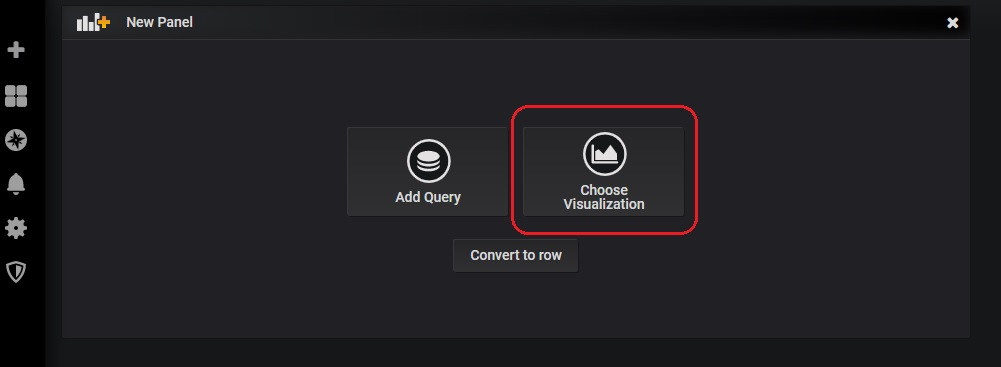
\includegraphics[scale=0.65]{img/plug-in/visual.jpg}
\caption{Chose Visualization button}
\end{figure}


	\item Finally, by pressing on the “Predire in Grafana” button, the user can use the plug-in.
	
\begin{figure}[H]
\centering
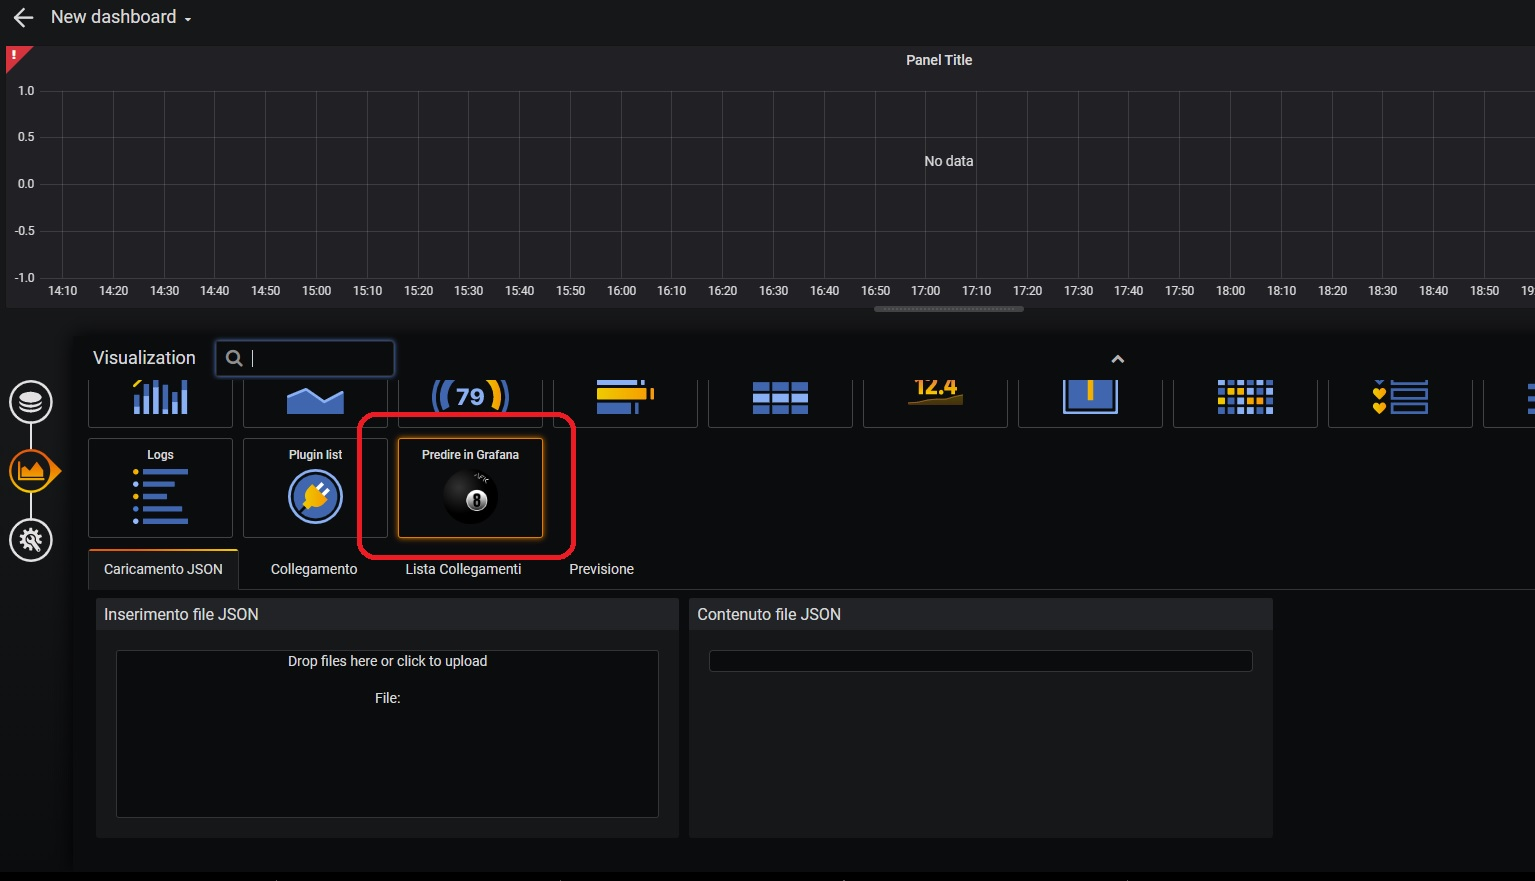
\includegraphics[scale=0.55]{img/plug-in/selection_ball.jpg}
\caption{"Predire in Grafana" Panel}
\end{figure}

\end{enumerate}

	
\subsection{Loading a JSON file}
The user can select the “Inserimento file JSON” button contained in the “Caricamento JSON” section.
This will open a window from which the JSON file can be selected.
Alternatively, the user can drag and drop the JSON file in the "Inserimento file JSON" section.
The content of the JSON file will be displayed in a panel called "Contenuto file JSON" to the right of the previously mentioned section.

\begin{figure}[H]
\centering
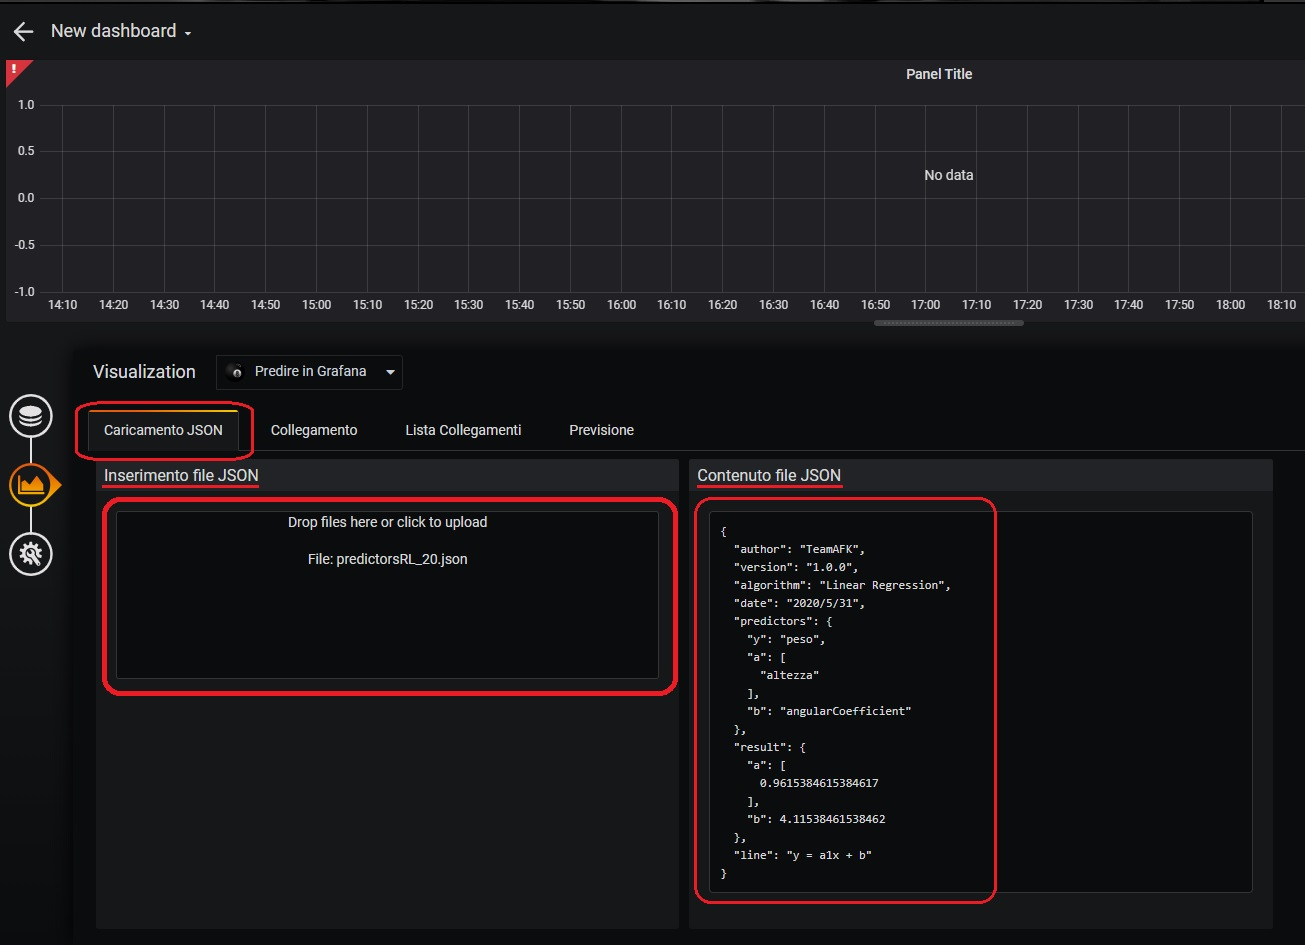
\includegraphics[scale=0.65]{img/plug-in/loading_js.jpg}
\caption{Loading window and displayed loaded JSON}
\end{figure}


\subsection{Connecting the nodes}
The portion of the software dedicated to the connection of the nodes can be accessed by selecting the "Collegamento" tab.
\begin{enumerate}
	\item The user can choose from the “Lista predittori” section which queries are to be associated with which nodes, by selecting a particular query to the right of a predictor: this can be done by opening the drop-down menu tagged with "Seleziona il nodo" and then selecting a query.
	Once all the nodes are connected, the user can select the "Inserisci collegamento" button and confirm the operation;
	
\begin{figure}[H]
\centering
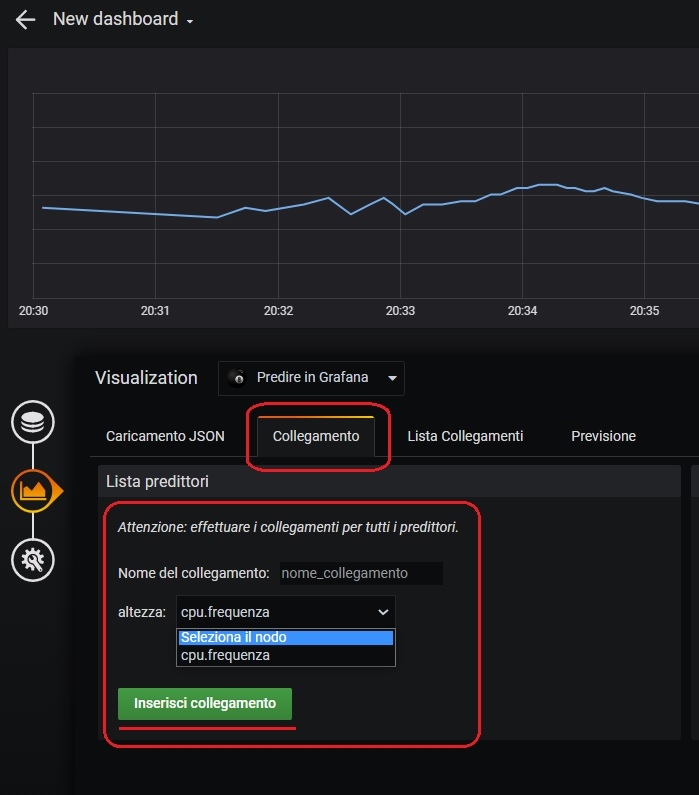
\includegraphics[scale=0.75]{img/plug-in/insert_node.jpg}
\caption{Node coupling (a)}
\end{figure}



\begin{enumerate}
\item Should the user have not filled all the required fields, an error message will be displayed on selection of the "Inserisci collegamento" button;

	
\begin{figure}[H]
\centering
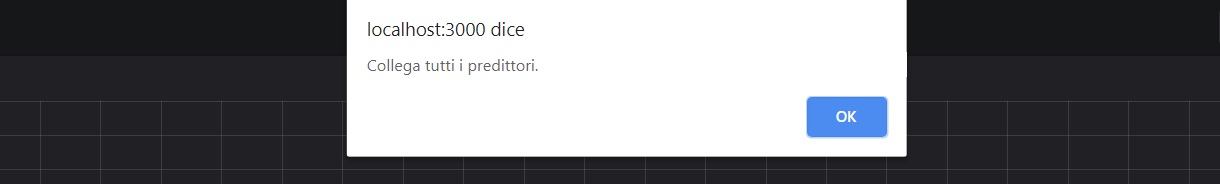
\includegraphics[scale=0.60]{img/plug-in/err_msg.jpg}
\caption{Node coupling error message}
\end{figure}

\item Once all the required fields are correctly chosen, a confirm message will be displayed. 

\begin{figure}[H]
\centering
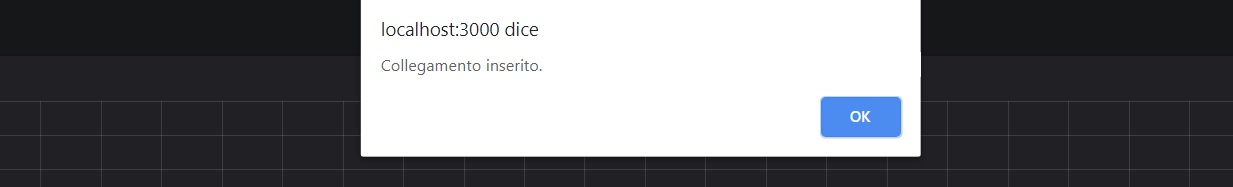
\includegraphics[scale=0.60]{img/plug-in/ok_msg.jpg}
\caption{Node coupling confirm message}
\end{figure}

\end{enumerate} 

	
	\item Maximum and minimum thresholds can be set in the “Impostazione soglie” section, by inserting numbers in the dedicated boxes and then selecting the "Conferma Collegamento" button.


\begin{figure}[H]
\centering
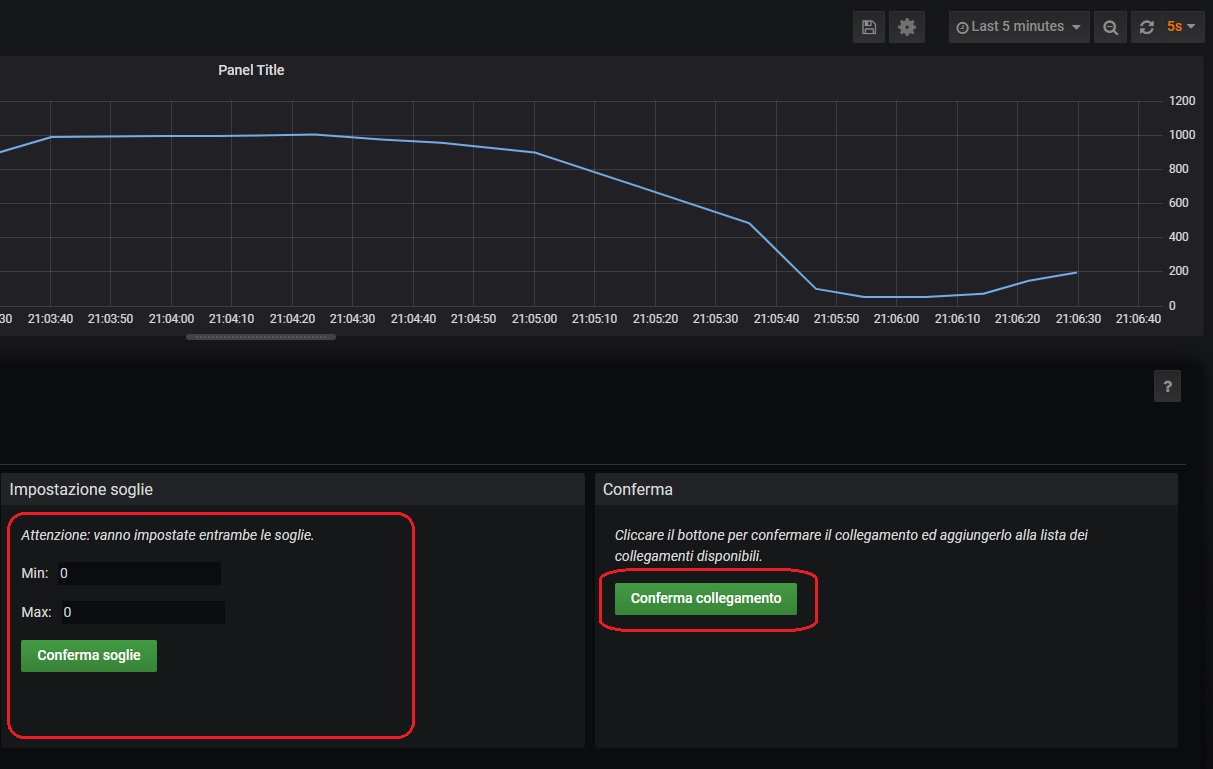
\includegraphics[scale=0.65]{img/plug-in/confirm.jpg}
\caption{Node coupling (b)}
\end{figure}

\end{enumerate}



\subsection{Modifying the connections}
In this section the user can view all the predictor-data stream connections that have been made. This section can be accessed by selecting the "Lista Collegamenti" tab.
The user can also modify the connection, by pressing on the "Modifica Collegamento" button, or delete it, by selecting the "Elimina Collegamento" button.

\begin{figure}[H]
\centering
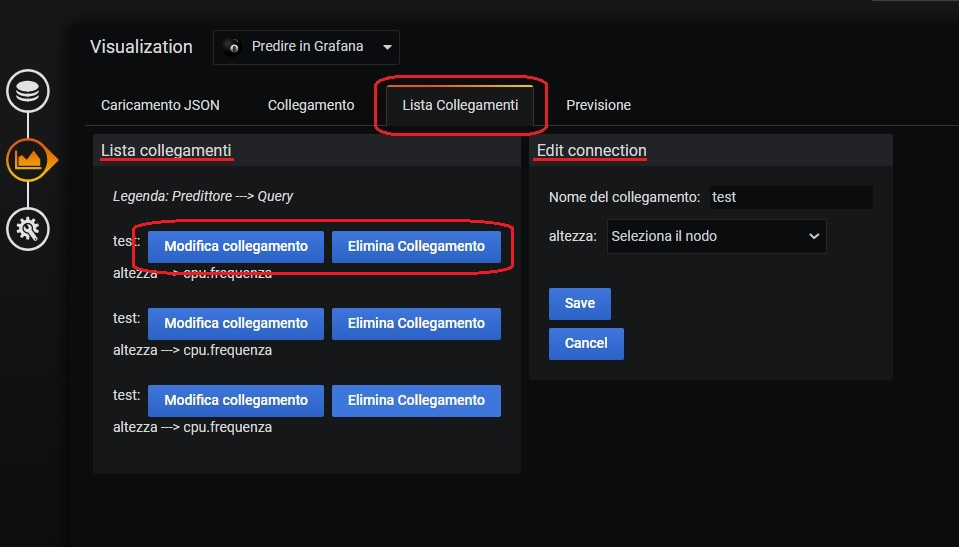
\includegraphics[scale=0.75]{img/plug-in/collegamento_node.jpg}
\caption{Node linking}
\end{figure}


\subsection{Prediction operations}
In this last section the user will be able to launch the prediction algorithms of the plug-in. This section is accessed by selecting the "Previsione" tab. Here the user will be able to select, in the top rigth corner, a temporal policy by choosing starting and ending dates and choosing how often to sample the data. The user  also has access to two buttons, one called "Avvia monitoraggio", which starts the prediction operations, and a second one named "Salva previsione", which saves the data collected up to the point it is pressed.\\

\begin{figure}[H]
\centering
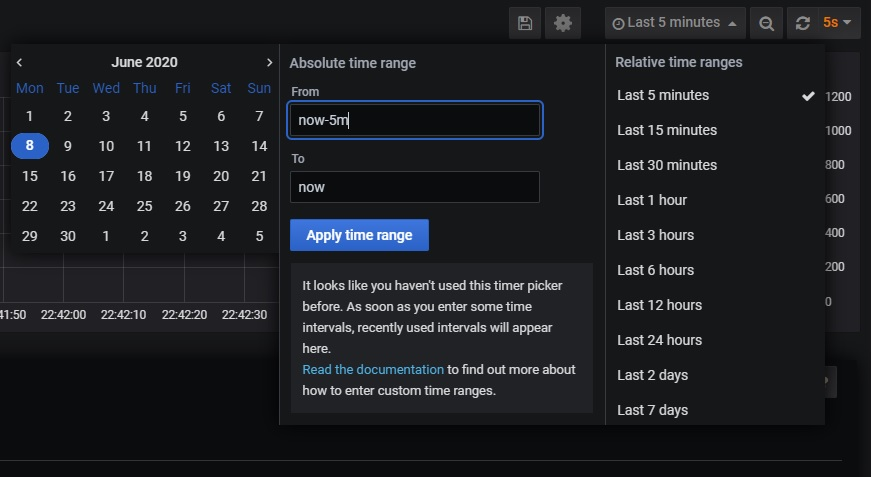
\includegraphics[scale=0.50]{img/plug-in/time_selector.jpg}
\caption{Time picker}
\end{figure}

When the prediction has been started, the "Avvia monitoraggio" button becomes "Interrompi monitoraggio", which, if pressed, will stop the monitoring.

\begin{figure}[H]
\centering
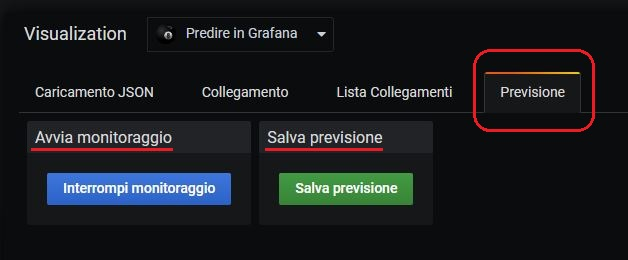
\includegraphics[scale=0.50]{img/plug-in/save_previsione.jpg}
\caption{Begin\textbackslash end data monitoring and predicton save}
\end{figure} 
 


\pagebreak
\section{File Structure}
\subsection{JSON structure}
The JSON files containing the configurations of the various prediction algoirthms must be structured in the following way

\subsubsection{Support Vector Machine}
\begin{itemize}
	\item \textbf{author}: file author;
	\item \textbf{version}: version of the application with the which the file was created;
	\item \textbf{algorithm}: states which algorithm was used for training, in this particular case "SVM";
	\item \textbf{date}: date on which the file was created;
	\item \textbf{predictors}: list of predictor tags;
	\item \textbf{result}: list of coefficients obtained from training.
\end{itemize}
\begin{figure}[H]
\centering
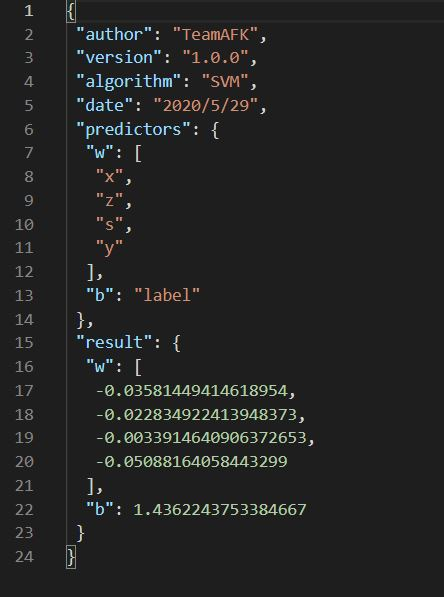
\includegraphics[scale=0.65]{img/json/jsonSVM.jpg}
\caption{Support Vector Machine JSON example}
\end{figure}
\newpage

\subsubsection{Linear Regression}
\begin{itemize}
	\item \textbf{author}: file author;
	\item \textbf{version}: version of the application with the which the file was created ;
	\item \textbf{algorithm}: states which algorithm was used for training, in this particular case "Linear Regression";
	\item \textbf{date}: date on which the file was created;
	\item \textbf{predictors}:  list of predictor tags;
	\item \textbf{result}: list of coefficients obtained from training;
	\item \textbf{line}: the equation of the Linear Regression.
\end{itemize}
\hspace{5cm}\\
\begin{figure}[H]
\centering
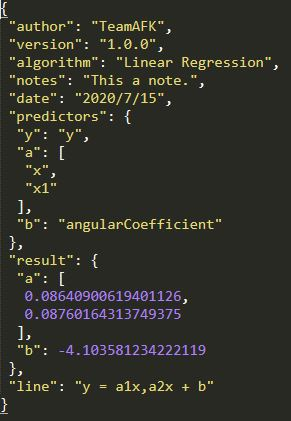
\includegraphics[scale=0.75]{img/json/jsonRL.jpg}
\caption{Linear Regression JSON example}
\end{figure}
\newpage
\subsection{CSV File structure}
The CSV files are structured based on which algorithm must be trained, RL or SVM.
Each column conains the values of the corresponding predictor\glo The first line  of each column must contain the tag associated to the particualar predictor. Depending on the case, one or more colums must be present for the predictors.

\begin{figure}[H]
\centering
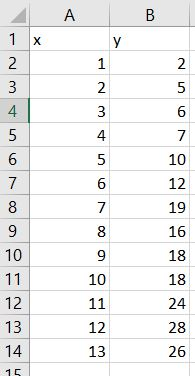
\includegraphics[scale=1]{img/json/csvfile.jpg}
\caption{CSV file example in Microsoft Excell}
\end{figure}

\pagebreak
\section{Reporting Errors}
Should anomalies or errors encountered during the execution of the plug-in or the training tool, it is possibile to report them ad the follwing mail address: \href{mailto:gruppoafk15@gmail.com}{gruppoafk15@gmail.com}.

\subsection{Reporting Training Tool errors}
In the object field the type of error must be stated in the following way: [Error][Training tool],
the body of the mail must contain the  following statements:

\begin{itemize}
	\item operating system version;
	\item training tool version;
	\item detailed explanation of the encountered. error
\end{itemize}

\begin{figure}[H]
\centering
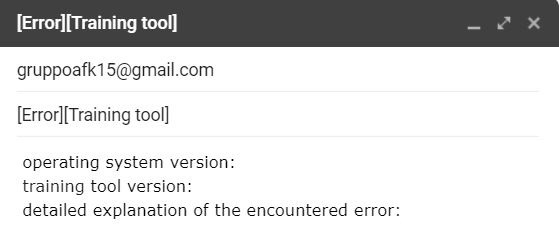
\includegraphics[scale=0.85]{img/mail/tool_mail.jpg}
\caption{Taining tool error mail template}
\end{figure}

\subsection{Reporting Plug-in errors}
To report Plug-in errors instead: the object field has to be compiled as such: [Error][Plug-in] and the body must contain the following statements:
\begin{itemize}
\item Grafana version;
\item plug-in version;
\item browser version;
\item operating system version;
\item  detailed explanation of the encountered.
\end{itemize}

\begin{figure}[H]
\centering
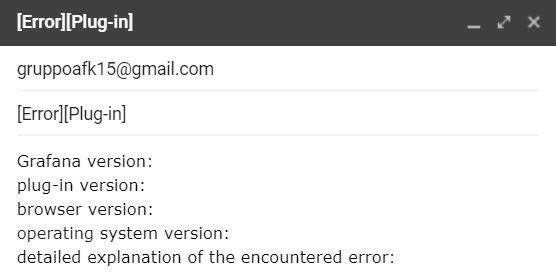
\includegraphics[scale=0.85]{img/mail/plug-in_mail.jpg}
\caption{Plug-in error mail template}
\end{figure}
\pagebreak

\appendix
\section{Glossary}

{\Large\textbf{G}\par}
\textbf{Grafana} \\
Open source platform which allows users to monitor data coming from various sources.

{\Large\textbf{M}\par}
\textbf{Machine Learning} \\
Machine learning is the study of algorithms which self improve through experience. Machine learning algorithms build mathematical models based on sample data known as "traning data". 

{\Large\textbf{P}\par}
\textbf{Predictor} \\
It is a function of the data, with the purpose of calculating predictions on one or more variables.

{\Large\textbf{R}\par}
\textbf{RL} \\
It is a method of estimating the expected value of a dependent variable given the values of the indipendent variables. 
It is defined as: $y = \alpha x + \beta $.

{\Large\textbf{S}\par}
\textbf{SVM} \\
It is a supervised machine learning model which uses classification algorithms to evaluate specific problems.

\end{document}